\documentclass[12pt]{article}
\usepackage{lingmacros}
\usepackage{tree-dvips}
\usepackage[english]{babel}
\usepackage{amsthm}
\usepackage{hyperref}
\usepackage{amsmath}

\newtheorem{theorem}{Theorem}[section]
\newtheorem{lemma}[theorem]{Lemma}
\newtheorem{claim}[theorem]{claim}
\usepackage[left=1in, right=1in, top=1in, bottom=1in]{geometry}

\usepackage{amsmath}
\usepackage{amssymb}
\usepackage{tikz}
\usepackage{mathtools}
\usetikzlibrary{automata,positioning,arrows}


\begin{document}
\begin{center}
\section*{Exercise 1 - Computational Models - Spring 2022}
\end{center}
\subsection*{Question 1}
Given a Boolean function $f : \lbrace0, 1\rbrace
^n \rightarrow \lbrace0, 1\rbrace$ and a boolean circuit C of size
$|C| = s$ that computes f, Lets proof that there existences of a boolean circuit $C'$ that's stand with the question property.
\begin{claim}
Any simple logic statement that uses $\vee$ or $ \wedge$ before $ \neg$ can be re-form to $\neg$ before $\vee$ or $ \wedge$ using one additional gate
\end{claim}
\begin{proof}
using De-Morgan law for  $ x,y \in \lbrace0, 1\rbrace$ : $\neg(x \vee y)$= $ \neg x \wedge \neg y$ and on the same way for $\neg(x \wedge y)$= $ \neg x \vee \neg y$, we apply the same statement using extra one gate in total. 
\end{proof}
using the claim above we can intuitive say that we need to "roll down the tree" all the NOT gates, and from quick indication I  can claim the following.
\begin{claim}
if $P$ have some cycle $C$ size $K$ that compute it $\Rightarrow$ three is some cycle $|C'|= |2K-1|$ that can computes $P$ where all the  $\neg$ gate's before any $ \wedge$ or $\vee$ gates
\end{claim}
\begin{proof}
the indication base case is given from claim0.1, so for some Atomic  $P$ where $P_i \in \lbrace0, 1\rbrace \Rightarrow$ in total $|K|$ simple gates we get:
\[  \neg (P_1 \vee P_2 \vee \dots P_n)\Rightarrow \neg P_1 \wedge \neg P_2 \wedge \dots \neg P_n  
\]
we can notice that now we need $|K|$ NOT gates and$|K-1|$ of $\wedge$ gates, and in total $|K+K-1|$  gates.
and all the  $\neg$ gate's before any $ \wedge$ gate's. \\Now lets $P_k$ be any boolean function that stand with the induction property,for some $x,y \in \lbrace0, 1\rbrace$ lets look at: 
\[ X=\neg (P_k\vee x)= \neg P_K \wedge \neg x, Y=\neg (P_k\wedge  y)= \neg P_K \vee \neg y\]
so in any case $X,Y$ can be written in $|2k-1|$ gates of $P_k$, additional NOT gate and one $\wedge$ or $\vee$ gate, in total $|2k-1+3|=|2k+2|$ under the induction assumption we know that $P$ have some $|C|=K$ that compute it ,so $C$ including the following $
\neg , \vee$ witch is size $|K+3|$ and can compute X
\end{proof}
on the same way we proof claim 0.2 we can get the same  property for  the $\wedge$ gate, so in total for some $f$ we can find for any appearance  of $\neg$ gate  $\in C$ , and each time apply De-Morgan law. based on claim 2 this new $|C'|$ hold the property (a)(b)(c).
\subsection*{Question 2}
For $f$ that has a circuit $C$ of size $m$ over $B_\ell$,
$C$ can be written as a binary tree with $m$ internal nodes. Each internal node is
labelled by a gate, and each leaf is labelled by a variable,
for each $v \in C$ lets $L_v: \lbrace0, 1\rbrace
^k \rightarrow \lbrace0, 1\rbrace $be the circut that accept language , according to Lupanov '58 theorem its can be expressed as language over DeMorgan basis ,using the result of exercise 2 at Recitation 1 ,we know that for such $L_v$ language there is some $C$ that can accept it when  $|C|=O(2^k)$
hence for $\forall v \in C \Rightarrow M|L_v|$ can be decided with some $C_m$ size $O(m2^\ell)$.
\subsection*{Question 3}
$\Longrightarrow$ Lets $M$ be an DFA such as $M=(Q,\sum,\delta,q_0,F)$ and assume that $M$ accept some $w \in \sum ^*
$ i.e $\hat{\delta}_{m}  (q_0,w) \in F$. using $\hat{\delta}_{m}$ definition ,lets $k_i$ be the state such as 
\[
\ \hat{\delta}_{m} (q_0,w)=k_{n}
\]
\[
\ \hat{\delta}_{m} (q_0,w)=\delta (\hat{\delta}_{m} (q_0,w_1,w_2\dots w_n-1),w_n)\Rightarrow k_{n-1}=\hat{\delta}_{m} (q_0,w_1,w_2\dots w_n-1)
\]
follow same proses for $n-2,n-3,\dots$ so for general $k_i$ on the "back-word" path
\[
\ \hat{\delta}_{m} (q_0,w_j)=\delta (\hat{\delta}_{m} (q_0,w_1,w_2\dots w_{j-1}),w_j)\Rightarrow k_{j-1}=\hat{\delta}_{m} (q_0,w_1,w_2\dots w_{j-1})
\]
hence $\forall k_i \in Q$ , $k_n \in F$,  $k_0=q_0$ and $\delta_m (k_{i-1},w_i)=k_i$ for $1 \leq i \leq n$ \\so we can claim that the sequence $k_1,k_2,\dots k_n$ stand with the property of the second equivalent DFA definition.\\\\
$\Longleftarrow$ Lets $M$ be an DFA such as $M=(Q,\sum,\delta,q_0,F)$ and we assume that\\ $\forall q_i \in Q$ , $q_n \in F$,$w_0=q_0$ and $\delta_m (q_{i-1},w_i)=q_i$ for some $w=w_1,w_2, \dots w_n$ and $q_1,q_2, \dots q_n$
\\ with the same way decribed above 
\[
\ \delta (q_0,w_1)=q_1,\hat{\delta_m}(q_0,w_1,w_2)=\delta ( \delta (q_0,w_1),w_2)=\delta( q_1,w_2)=q_2,
\]
in general
\[
\ \hat{\delta_m}(q_0,w_1,\dots ,w_j)=\delta ( \hat{\delta_m} (q_0,w_1,\dots ,w_{j-1}),w_j)=q_j
\]
\[
\ \hat{\delta_m}(q_0,w_1,\dots ,w_n)=\delta ( \hat{\delta_m} (q_0,w_1,\dots ,w_{n-1}),w_n)=q_n \in F
\]
and we proof that both definition are equivalent
\subsection*{Question 4}
\begin{figure}[ht] % ’ht’ tells LaTeX to place the figure ’here’ or at the top of the page
\centering % centers the figure
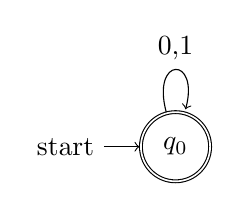
\begin{tikzpicture}
\node[state, accepting,initial]  (q1) {$q_0$};

\draw (q1) edge[loop above] node{0,1} (q1);
\end{tikzpicture}
\caption{ DFA (a) $\Sigma^*$}
\label{fig:my_label}
\end{figure}

\begin{figure}[ht] % ’ht’ tells LaTeX to place the figure ’here’ or at the top of the page
\centering % centers the figure
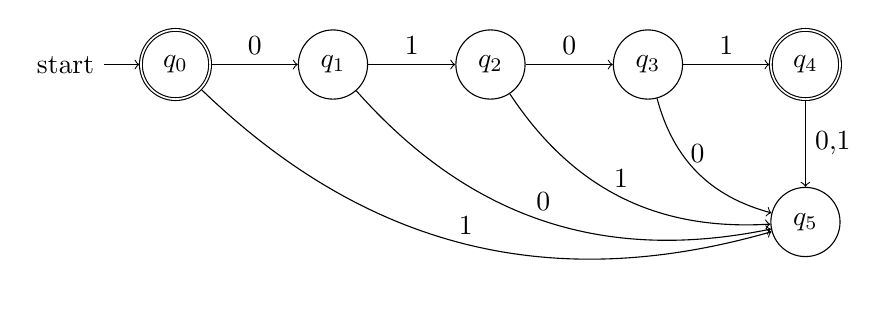
\begin{tikzpicture}
\node[state, accepting,initial]at (0, -3) (q0) {$q_0$};
\node[state, right of=q0,xshift=1cm] (q2) {$q_1$};
\node[state, right of=q2,xshift=1cm] (q3) {$q_2$};
\node[state,, right of=q3,xshift=1cm] (q4) {$q_3$};
\node[state,accepting, right of=q4,xshift=1cm] (q5) {$q_4$};
\node[state,, below of=q5,yshift=-1cm] (q6) {$q_5$};
\path[->]
(q0) edge[above] node{0} (q2)
(q2) edge[above] node{1} (q3)
(q3) edge[above] node{0} (q4)
(q4) edge[above] node{1} (q5)
(q0) edge[bend right,above] node{1} (q6)
(q2) edge[bend right,above] node{0} (q6)
(q3) edge[bend right,above] node{1} (q6)
(q4) edge[bend right,above] node{0} (q6)
(q5) edge[right] node{0,1} (q6)
;;\end{tikzpicture}
\caption{DFA (b) $\lbrace \epsilon ,0101\rbrace$}
\label{fig:my_label2}
\end{figure}

\begin{figure}[ht] % ’ht’ tells LaTeX to place the figure ’here’ or at the top of the page
\centering % centers the figure
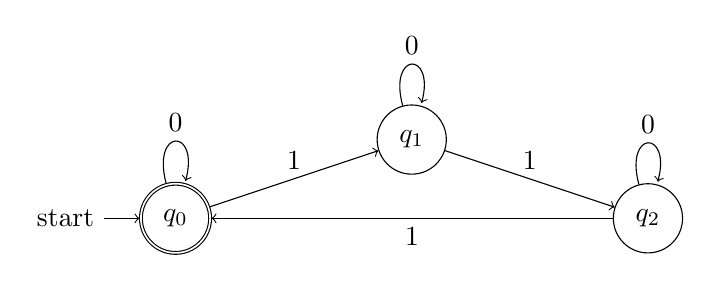
\begin{tikzpicture}
\node[state, accepting,initial]at (0, -4) (q0) {$q_0$};
\node[state, above of=q0,xshift=3cm] (q2) {$q_1$};
\node[state, right of=q0,xshift=5cm] (q3) {$q_2$};

\path[->]
(q0) edge[above] node{1} (q2)
(q2) edge[above] node{1} (q3)
(q3) edge[below] node{1} (q0)
(q0) edge[loop above] node{0} (q0)
(q2) edge[loop above] node{0} (q2)
(q3) edge[loop above] node{0} (q3)
;;\end{tikzpicture}
\caption{DFA (c) $\lbrace w| \#_1w \text{ mod 3 } \equiv 0\rbrace $ }
\label{fig:my_label2}
\end{figure}
\pagebreak
\subsection*{Question 5}
Given n, Lets formalize the language \[L_n=\lbrace w0w_n | w \in \lbrace 0,1\rbrace^* \wedge   w_n \in \lbrace 0,1\rbrace^{n-1}
\rbrace
\]
lets present NFA $N=(Q,\Sigma,\delta,S,F)$ that accept $L_n$ , we know that any NFA can be transform to DFA .\\
\[ Q=\lbrace q_0,q_1\dots ,q_{n} \rbrace 
,\Sigma =\lbrace 0,1\rbrace
,S =\lbrace q_0\rbrace 
,F =\lbrace q_{n}\rbrace \]
\[   
\delta(q_i,\sigma) = 
     \begin{cases} 
      \lbrace q_0,q_1   \rbrace  &\quad\text{if } q_i=q_0 \wedge \sigma=0 \\
       \lbrace q_0   \rbrace  &\quad\text{if     } q_i=q_0 \wedge \sigma=1 \\
        \lbrace q_{i+1}   \rbrace  &\quad \text{if } 0<q_{i}<q_n \forall \sigma \in \Sigma \\
          \phi  &\quad\text{if } q_i=q_n  \forall \sigma \in \Sigma \\ 
     \end{cases}     
\]
\begin{claim}
N accept $L_n$
\end{claim}
\begin{proof}
$w \in L_n \Leftrightarrow$ 
\[ w \in \lbrace w0w_n | w \in \lbrace 0,1\rbrace^* \wedge   w_n \in \lbrace 0,1\rbrace^{n-1}\rbrace
\Leftrightarrow
\exists \hat{w} \in \Sigma^*.\exists \sigma \in \lbrace 0\rbrace
.w_n \in \lbrace 0,1\rbrace^{n-1}
\]
\[
\Leftrightarrow
\exists \hat{w} \in \Sigma^*.\exists \sigma \in \lbrace 0\rbrace
.\hat{\delta}_w(q_1,w_{n})\in Q
\Leftrightarrow
\exists  \hat{w} \in \Sigma^*.\exists \exists \delta(q_0,q_1) ,\hat{\delta}_w(q_1,w_{n}))\in Q
\]
\[
\Leftrightarrow
\exists  \hat{w} \in \Sigma^*.\exists  \hat{\delta}(q_0,q_n)\in Q
\Leftrightarrow
\exists \exists \dots q_i,q_j\in Q.\exists  \hat{\delta}(q_0,q_n)\in F
\]
\[
 \Leftrightarrow \delta(\hat{\delta}_w(q',q_n),\sigma)\exists q' \in Q
 \forall \sigma \in \Sigma .\hat{\delta}(q_0,q_n)\in F \Leftrightarrow
 \phi.(q_0,q_n)\in F
 \Leftrightarrow
 (q_0,q_n)\in L(N)
\]
to be honest i'm not relay sure about the last few equivalence :)
\end{proof}
Now lets show N as DFA 
\[ Q_m=\lbrace [R]|R \in Q \rbrace 
,\Sigma =\lbrace 0,1\rbrace
,\delta_0 = q_0
,F_m =\lbrace [R]|R \cap Q \neq \phi \rbrace,\delta_m([R],\sigma) =\cup_{q \in R} \delta(q,\sigma )
 \]
 
\subsubsection*{Question 5 (b)}
\begin{claim}
All regular languages is closed under $\backslash$ with a
any regular language.
\end{claim}
\begin{proof}
Lets $L_1$ and $L_2$ be regular, using the regular opertor  we know already, we can immediately claim that following holds 
\[ L_1 \cap \overline{L_2} \Rightarrow L_1\backslash L_2 \text{ is regular language} 
\]
\end{proof}
\subsection*{Question 6}
Let  $A=(Q,\sum,\delta,q_0,F)$ be a DFA, and let $w_1,w_2 \in \Sigma^*$ be words such that $\hat{\delta}(q_0, w_1) = \hat{\delta}(q_0, w_2).$
Lets proof that for every word $ w \in \Sigma^*$
it holds that $w_1w \in L(A) \Leftrightarrow w_2w \in L(A) $ 
now we set some $q_k$ such as \\$\hat{\delta}(q_0, w_1) = \hat{\delta}(q_0, w_2)=q_k \in Q$. now we construct new $A_1$ and $A_2$ in the following way:
\[ A_1=(Q,\Sigma ,\delta,q_0,q_k=F_1),
A_2=(Q,\Sigma ,\delta,q_k,F_2=F)
\]
we can notice that  $\hat{\delta}(q_0, w_1) = \hat{\delta}(q_0, w_2) \in L(A_1)$ ,and for some $w$ such as $w \in L(A_2)$ we get 
\[
w \in L(A_2) \Leftrightarrow  \hat{\delta}(q_k, w) \in F_2
 \Leftrightarrow  \hat{\delta}(q_k, w) \in F
 \]
 \[
  \Leftrightarrow  q_k \in F_1, \hat{\delta}(q_k, w)\in F  
  \]
 \[
  \Leftrightarrow \forall w'\in L(A_1).\hat{\delta} (\hat{\delta}(q_0,w')),w)\in F
   \]
 \[
    \hat{\delta} (\hat{\delta}(q_0,w_1)),w)\in F 
   \Leftrightarrow \hat{\delta} (\hat{\delta}(q_0,w_2)),w)\in F 
\]
 \[
   w_1w\in L(A)
   \Leftrightarrow    w_2w\in L(A)
\]
\subsubsection*{Question 6 (b)}
Let n be a number and let A be a DFA such that $L(A) = \lbrace0^
i1^
i
: 0 \leq
i \leq n\rbrace.
$
now follow the hint
\begin{claim}
$\hat{\delta}(q_0,0^i) \neq \hat{\delta}(q_0,0^i) $
for any $i\neq j$
\end{claim}
\begin{proof}
lets assume that $\hat{q}=\hat{\delta}(q_0,0^i) = \hat{\delta}(q_0,0^j) $ and without any loss of generality $i<j$ .from  A definition we know that $w_i:= 0^i1^i ,w_i:= 0^j1^j \in L(A)$ i.e for $\hat{\delta}(\hat{\delta}(q_0,0^j),1^i )$ we can get to for some $q\in F$. now lets look at 
 \[\hat{\delta}(q_0,w)\in F \Rightarrow\  \hat{\delta}(\hat{\delta}(q_0,0^i),1^j )=\hat{\delta}(\hat{q},1^i )
\]
under the assuming we lets look at 
\[\hat{\delta}(\hat{q},1^i )=\hat{\delta}(\hat{\delta}(q_0,0^j),1^i )=\hat{\delta}(q_0,0^j1^i)\in F
\]
and we got an contradiction.

\end{proof}
Hence the claim above hold for any $i\neq j$ and in total we find that A  has at least n accepting state.

  \end{document}